\renewcommand{\thefigure}{\textsc{a}\arabic{figure}}
\renewcommand{\theequation}{\textsc{a}\arabic{equation}}
\renewcommand{\thetable}{\textsc{a}\arabic{table}}
\setcounter{figure}{0}
\setcounter{equation}{0}

%\chapter{Appendix to chapter 3}

\chapter{Appendix to chapter 5}

\section{Scenario modeling vignette}
Here is presented a vignette with 50 model simulations in a fictional setting (Location X) with nine counties (named A through I) in demonstrative intervention scenarios from January 31 to December 31, 2020. In this vignette, a walk through is offered on how to set up and run the pipeline, demonstrate some of the spatial and temporal features for modeling non-pharmaceutical interventions, and display some of the plotting functions useful for summarizing the model output.

To run the model, users will require a second GitHub repository specific to their model location. A template for such a spatial repository may be found at “\verb|COVID19_Minimal|” (\url{github.com/HopkinsIDD/COVID19_Minimal}), and complete details on downloading and running the model are available in the template’s wiki at \url{github.com/HopkinsIDD/COVID19_Minimal/} wiki.

Once a working environment is setup, the next step is to create a configuration file to describe the model specifications. A skeleton configuration file is included in the \verb|COVID19_Minimal| template, and the full configuration file accompanying the results of this vignette is in the “Supplementary Material”.

First, the broad parameters of the run, such as the date range covered and the number of simulations to run are provided (see first section in “Supplementary Material”, Example YAML Configuration File).

Next the spatial setup information identifying the location of files containing geographic data and the geographic targets for modeling are described. The \verb|spatial_setup| section of the configuration file identifies a geographical data (geodata) file that contains the population data for each county or administrative subunit in the location(s) of interest and a mobility matrix file that contains the daily trip counts for each pair of counties. Users may employ the R scripts “\verb|build_US_setup.R|” or “\verb|build_nonUS_setup.R|,” which are provided with the repository, to generate compatible geodata and mobility matrix files. For users modeling non-US settings, the Github repository “\url{COVID-19-Mobility-Data-Network/mobility}” can be used to fit real-time or sparse travel data with mobility models in order to generate similarly compatible mobility matrixes\cite{Giles:COVID19MobilityDataNetworkMobilityV0:2020,Giles:MobilityPackageModeling:2020}.

In situations with high cross-border mobility, it may be important to model a region larger than the location of interest in order to appropriately capture disease transmission risk in a given location. Here, Locations X, Y, and Z are modeled even though Location X is the sole location of interest:
\begin{lstlisting}[language=yaml]
spatial_setup: 
  base_path: data/location-x ## base path to spatial files 
  setup_name: location-x ## spatial folder name 
  geodata: geodata.csv ## path to geodata file with modeled geoids 
  mobility: mobility.csv ## path to mobility matrix 
  popnodes: pop ## column name of population in geodata 
  nodenames: geoid ## column name of unique location identifiers in geodata 
  modeled_states: 
    - X 
    - Y 
    - Z
\end{lstlisting}

The locations of the seeding files are then specified (see seeding section in “Supplementary Material”, Example YAML Configuration File), with a separate section to describe the air importation model parameters as appropriate (see importation in “Supplementary Material”, Example YAML Configuration File).

Next, the parameters that determine the course of the disease are choosen. The seir section of the configuration file defines parameters used in the SEIR disease transmission model, including the level of population mixing (where 1 is homogeneous mixing, and <1 is heterogeneous), the incubation period of the virus, the infectious period, and the baseline basic reproductive number R0. These values may be fixed or drawn randomly from a distribution, according to the configuration file:
\begin{lstlisting}[language=yaml]
seir: 
  parameters: 
    alpha: 1 ## mixing coefficient 
    sigma: 1 / 5.2 ## inverse of the incubation period in days 
    gamma: ## inverse of the infectious period in days 
      distribution: uniform 
      low: 1 / 6 
      high: 1 / 2.6 
    R0s: ## baseline basic reproductive number 
      distribution: uniform 
      low: 2 
      high: 3
\end{lstlisting}

Typically sigma and gamma are parameterized in our model with estimates of the range of the serial interval (SI) or generation time, such that
\begin{equation}
\text{SI}=\frac{1}{2}\left(\frac{1}{\gamma }\right)+\frac{1}{\sigma },
\end{equation}
which assumes that the average infection occurs halfway through an index case’s infectious period.

The next step is defining the modeled intervention scenarios. Here, five scenarios are considered in our vignette example: (1) a no intervention scenario (named Uncontrolled), in which R0 remains unchanged over the course of the outbreak; (2) social distancing measures with fixed effectiveness in place from March 19 to December 31 (\verb|SocialDistancing_fixed|); (3) social distancing measures with declining compliance, which were modeled as 10\% reductions in effectiveness every 2 weeks beginning March 19 (\verb|SocialDistancing_fatigued|); (4) social distancing measures following a 3-week on–off “pulsing” cycle from March 19 to August 12 (\verb|SocialDistancing_pulsed|); and (5) social distancing measures with spatial heterogeneity (\verb|SocialDistancing_checker|), where three of nine counties implement social distancing measures with fixed effectiveness from March 19 to December 31.

%\begin{mybox}{Initial parameters}
\marginnote{\textsc{Initial parameters}The serial interval represents which is the interval between two subsequent infections. For SARS-CoV-2, the serial interval was estimated to be in range $6.5-8.2$, from: \fullcite[][tab. S4]{Bi:EpidemiologyTransmissionCOVID19:2020}. 

The basic reproductive number $R_0$ -- the number of newly infected caused by an infecteds in a fully susceptible population, has been estimated in the range 2 -- 3. From: \fullcite{Riou:PatternEarlyHumantohuman:2020}. This very early work also characterize $R_0$ and the dispersion of the number of secondary cases as important epidemic characteristic.
}

An intervention may be specified in a single block for all model locations, as in the case of the \verb|SocialDistancing_fixed| scenario, or for unique location identifiers (“geoids”) as in the \verb|SocialDistancing_checker| scenario:
\begin{lstlisting}[language=yaml]
SocialDistancing_fixed: ## scenario name 
  template: ReduceR0 
  period_start_date: 2020-03-19 ## intervention start date 
  period_end_date: 2020-12-31 ## intervention end date 
  value: ## randomly draw an intervention effectiveness value 
         ##from a uniform distribution between .71 and .83 
    distribution: uniform 
    low: .71 
    high: .83 
SocialDistancing_checker: 
  template: ReduceR0 
  affected_geoids: ["County B", "County E", "County F"] 
  ## ^ matches location IDs in geodata file 
  period_start_date: 2020-03-19 
  period_end_date: 2020-12-31 
  value: 
    distribution: uniform 
    low: .71
    high: .83
\end{lstlisting}

Other intervention scenarios require multiple blocks to be stacked together, as in the case of the \verb|SocialDistancing_pulsed| scenario, shown in truncated form below: 

\begin{lstlisting}[language=yaml]
SD_Pulse1: 
  template: ReduceR0 
  period_start_date: 2020-03-19 
  period_end_date: 2020-04-08 
  value: 
    distribution: uniform 
    low: .71 
    high: .83 
SD_Pulse2: 
  template: ReduceR0 
  period_start_date: 2020-04-30 
  period_end_date: 2020-05-20 
  value: 
    distribution: uniform
    low: .71 
    high: .83 
# [... SD_Pulse3 and SD_Pulse4 ...]
SocialDistancing_pulsed: 
  template: Stacked 
  scenarios: 
    - SD_Pulse1 
    - SD_Pulse2
    - SD_Pulse3
    - SD_Pulse4
\end{lstlisting}

Then, the health outcome risk specifications are set up. In the hospitalization section of the configuration file, it is specified whether the model calculates health outcome risks with age-adjusted estimates, the average infection fatality ratios (IFR), and the time delays between different health outcomes. The time delays are modeled with lognormal distributions and parameterized with the log median and log standard deviation. For ease of use, a table of estimates found in the literature is provided in tab. S2 of the postprint.

After the simulation runs complete, wrapid summaries of the results are produced using R Markdown templates provided by the report.generation package. The report section of the configuration file specifies scenario labels and colors, IFR scenario labels, and table display dates. These settings, along with other model parameters, can be loaded into a technical report template.

Here it is described how the \verb|state_report| template in the report.generation package can be used to display our model results as an example. The full template-generated report linked to this vignette is provided in the “Supplementary Material” (Example Report). First, the configuration file is loaded to pull in the model settings and file paths. Then, a number of predefined functions to load and plot the data are used.

For example, one standard report figure compares time series of the daily number of hospital beds needed across intervention scenarios (fig.~\ref{fig:pipeline-seir}) using the \verb|load_hosp_geocombined_totals| and \verb|plot_ts_hosp_state_sample| functions from the report.generation package in order to load and plot the data. To plot variations of these figures, one only need to change which health outcome variable is specified in \verb|plot_ts_hosp_state_sample|.

While fig.~\ref{fig:pipeline-seir} displays aggregate results, our reports also provide location-specific risk and logistical outputs at the county- or administrative subunit-level. For example, the age-adjusted infection fatality ratios and risk of ICU admission among hospitalized infections for the modeled counties within the distribution of all counties in the United States are presented in fig.~\ref{fig:pipeline-outcome}\textsc{a,b}. Using the \verb|load_hosp_geounit_relative_to_threshold| and \verb|plot_needs_relative_to_threshold_heatmap| functions from report.generation, the potential need for beds in excess of health system capacity by model location is displayed in our reports (fig.~\ref{fig:pipeline-outcome}\textsc{c}). Values of the location-specific healthcare capacity, represented by the number of staffed hospital, acute care, or intensive care beds available and/or number of ventilators available, are user-defined; these can be based on assumptions of the average availability per person or input from data where available.

A map of model outputs makes it easier to visualize spatial and temporal heterogeneity in different intervention scenarios (fig.~\ref{fig:pipeline-map}). This functionality is provided in the \verb|load_cum_inf_geounit_dates| and \verb|plot_geounit_map| functions in the report.generation package.

Each report template is equipped to load static R Markdown reference chunks, which is pre-written and provided with the package. These chunks provide details on our methods, limitations, and key references, pulling in parameters from the configuration file as needed.



\chapter{Appendix to chapter 6}

\section{Comment on the simplifications}
\paragraph{Discussion on Simplification (a).}
Realistically, vaccinations will occur at least eight hours per day. Our assumption, while justified as a computationally convenient approximation of reality, is not a priori worse than assuming that vaccine administration takes place over the whole day. More refined approximations, while in principle possible, pose severe issues because of the nature of the system dynamics. While for most initial values the system dynamics can be easily simulated with time-continuous vaccinations, the system becomes stiff by construction once almost the entire population has been vaccinated. In this case, numerical integration errors can drive the size of some compartments to be negative, which violates the model assumptions and makes the result of the numerical integration meaningless. The main issue in this case is that the optimizer will exploit these inaccuracies in order to reduce the cost. Therefore, this issue is much more evident when solving optimal control problems than when simply simulating the system dynamics. Some simple approaches to tackle this issue are investigated, but no technique yielded satisfactory performances. It is our impression that ad-hoc integration strategies will be required in order to reliably simulate and optimize dynamics with continuous vaccination rates. While this will be the subject of future research, the results obtained with the current approximation have yielded sufficient accuracy.

\paragraph{Discussion on Simplification (b).}
This simplification has been proposed in~\cite{Savorgnan:MultipleShootingDistributed:2011} as an approach to solve distributed optimal control problems by means of multiple shooting. In the original version, the coupling variable $z$ is not necessarily piecewise constant, but rather piecewise polynomial. In simulations of this problem, the piecewise constant parametrization has been observed to yield sufficient accuracy.

The dynamics of each node are discretized using an explicit Runge-Kutta integrator of order four, with $50$ integration steps per day. Alternative integrators such as explicit Euler, or implicit Runge-Kutta integrators, yielded similar results. Furthermore, in order to verify the accuracy of the integrator and the impact of the introduced simplifications on the solution accuracy, the system is simulated in open-loop, i.e. the optimal control trajectory is applied to the full model starting from the initial condition provided by the data assimilation scheme.

\paragraph{Discussion on Simplification (c).} The mobility matrix is sparsified by pruning element below a threshold (see fig.~\ref{figSI:mobility_simplification}). This operation reduces the number of connection between nodes. Also in this case, the introduced simplification has been verified through numerical simulations to have a small impact on the prediction and control accuracy.

\begin{figure*}
\centering
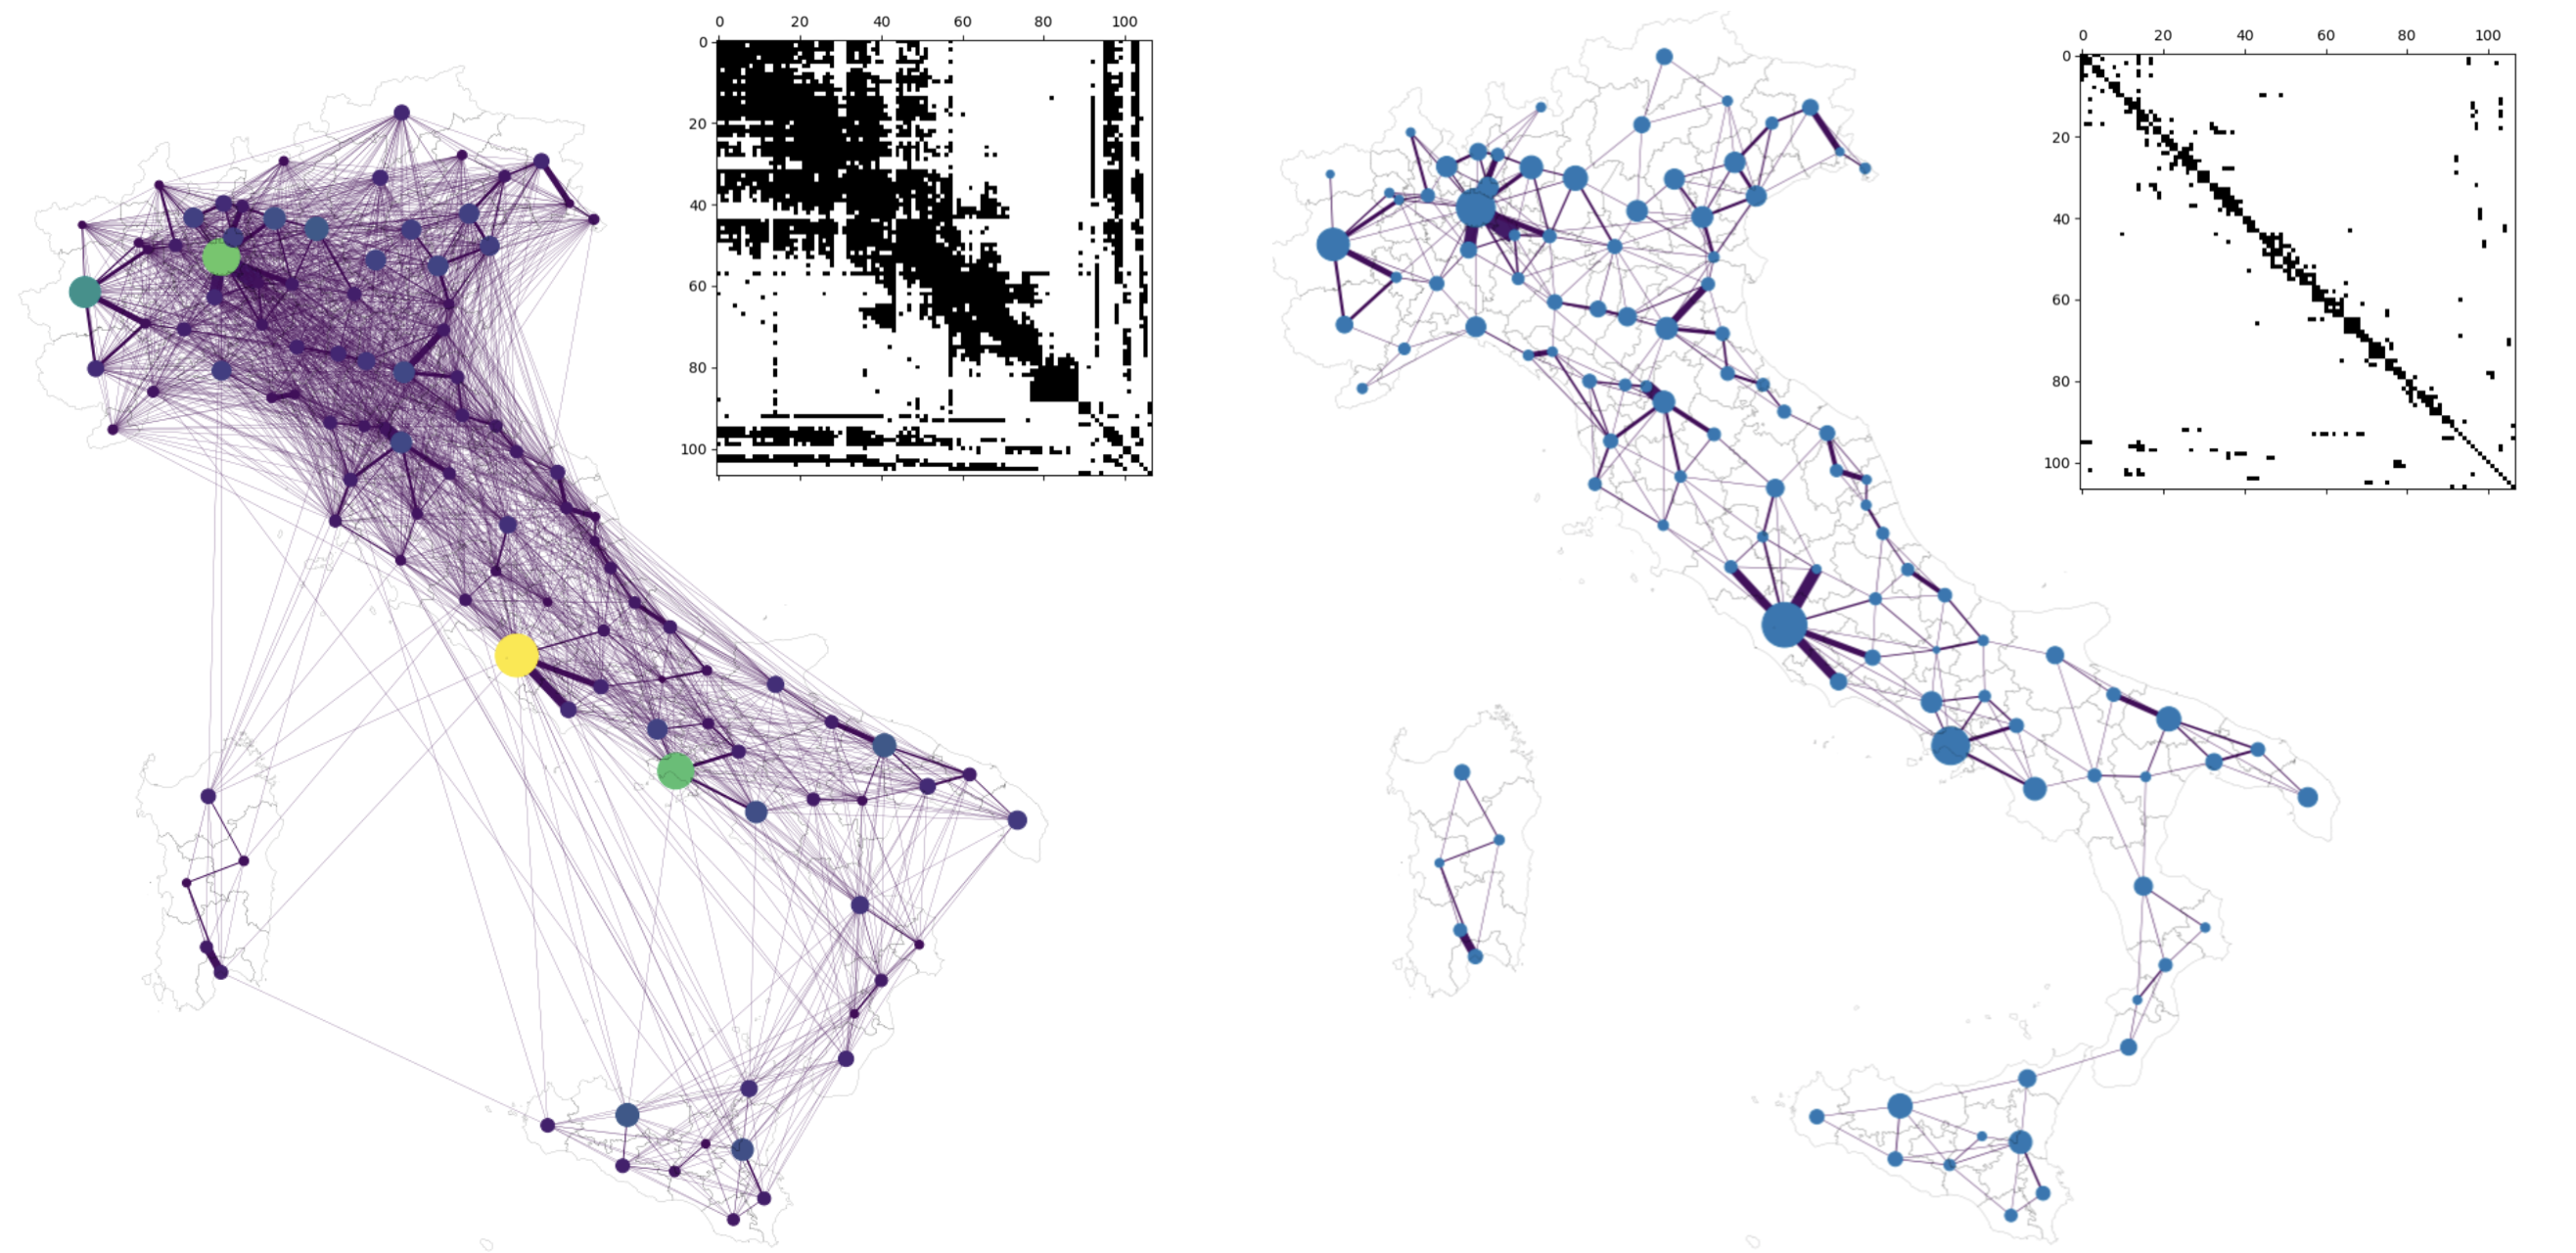
\includegraphics[width=\textwidth]{fig_italy-ocp/figuresSI/mobsimplification.png}
\caption[Simplification of the mobility matrix to obtain a sparse and tractable problem]{Simplification of the mobility matrix to obtain a sparse and tractable problem. After the optimization, the effectiveness of the optimal control strategy is assessed on the full model.} \label{figSI:mobility_simplification}
\end{figure*}

\paragraph{Possible further improvements} Applying optimal control in open loop, i.e., solving the optimization problem once and applying the control input over the whole time interval, may lead to poor performance due to model inaccuracy and external perturbations. A common remedy consists in closing the loop by repeatedly solving the OCP by using the most updated information on the initial states. This is the principle behind Model Predictive Control (MPC)~\cite{Rawlings:ModelPredictiveControl:2017}. In this context, the state would be estimated on a daily, weekly, or monthly basis so as to solve again the OCP and correct the optimal strategy.


%% ***********************************************************************************************
%\section{Data assimilation and model parameters}
%% ***********************************************************************************************
%\begin{figure*}
%    \centering
 %   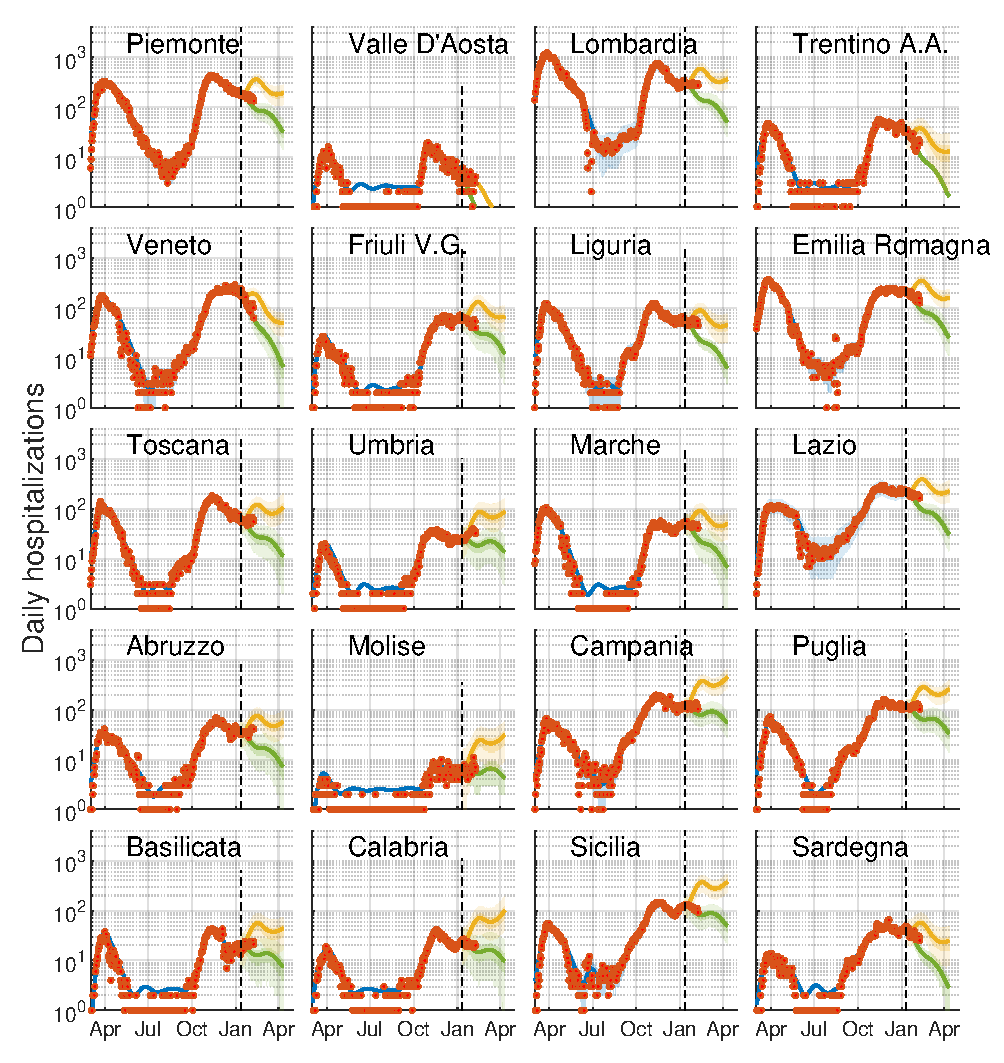
\includegraphics[width=1\textwidth]{fig_italy-ocp/figuresSI/DA_all_sim/hosp.pdf}
  %  \caption[Modeled daily hospitalizations the against hospitalization data]{Modeled daily hospitalizations (blue) versus hospitalization data (red dots), regional detail of fig. 2.A in the main text. The optimistic and pessimistic transmission scenarios are represented in green and yellow, respectively.}
%    \label{fig:SI_DA1}
%\end{figure*}
%\begin{figure*}
%    \centering
%    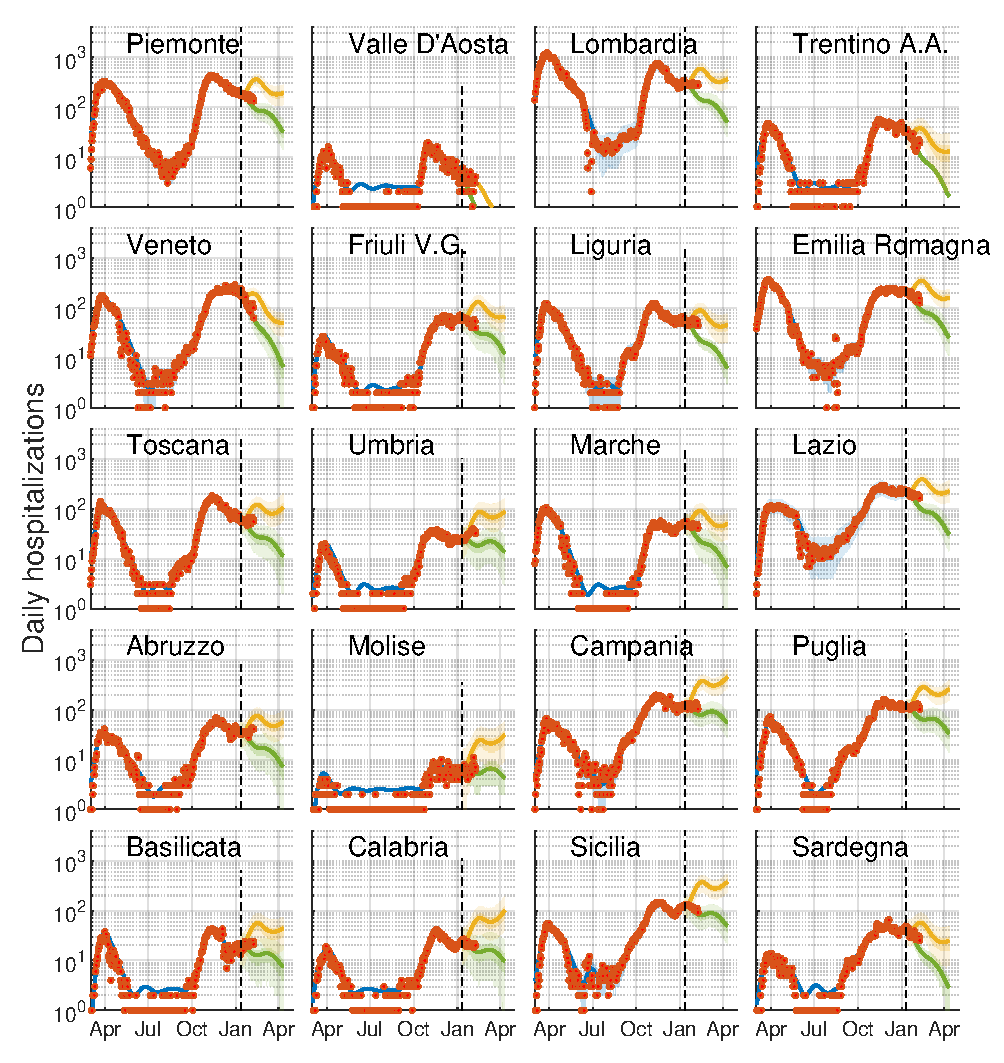
\includegraphics[width=1\textwidth]{fig_italy-ocp/figuresSI/DA_all_sim/incidence.pdf}
%    \caption[Modeled daily incidence against the daily reported cases]{Modeled daily incidence (blue) versus the daily reported cases (red dots), regional detail of fig. 2.B in the main text. The optimistic and pessimistic transmission scenarios are represented in green and yellow, respectively.}
%    \label{fig:SI_DA2}
%\end{figure*}

%The regional transmission rates are the main parameters governing the force of infection of the model and, thus, the daily exposed individuals. To better track possible changes in the transmission rates, w- adopt a data assimilation strategy based on an iterative particle filter\cite{Manoli:IterativeParticleFilter:2015} used on a moving window of 14 days. The filter starts considering $N_r=1000$ model realizations at time $t_0$ (February 21st, 2020), whose state variables are $x_0^{(j)}, j=1,\dots, N_r$, where the superscript $(j)$ is the realization index and the subscript is the temporal index. Each realization is associated with a parameter combination that is randomly sampled from the posterior distribution evaluated in\cite{Bertuzzo:GeographyCOVID19Spread:2020}, indicated with $\theta^{(j)}$. Possible spatial heterogeneities in regional transmission on a given day $t_k$ are obtained multiplying the transmission parameter by a coefficient $\phi_{k,i}^{(j)}$, where $i$ is the region's index. At time $t_0$, the coefficients $\phi_{0,i}^{(j)}$ are sampled from a truncated normal distribution (mean $\mu_0=1$, standard deviation 0.4, bounds $0.8\mu$-$1.2\mu_0$).
%At time $t_k$, w- assume to know the state variables $x_k^{(j)}$ and coefficients $\phi_{k,i}^{(j)}$, the latter having ensemble mean $\mu_{k,i}$. To update state variables and coefficients at time $t_{k+1}$, w- consider the observations (daily hospitalizations) collected in a temporal window of $\tau=14$ days, $(t_k,t_{k}+\tau$. New coefficients from the truncated normal distribution (mean $\mu_k=1$, standard deviation 0.4, bounds $0.8\mu_k$-$1.2\mu_k$) are sampled at time $\tau=t_0+14$ days.  For each realization, w- run the model during the window of 14 days, assuming that the coefficients change linearly for a week, from  $\phi_{0,i}^{(j)}$ to $\tilde{\phi}_{0,i}^{(j)}$, and remain constant afterwards.
%The regional likelihood of each realization is then evaluated during these two weeks considering that the daily hospitalizations follow a gamma distribution (as in\cite{Bertuzzo:GeographyCOVID19Spread:2020}). 
%A resampling step (systematic resampling , see, e.g.\cite{Douc:ComparisonResamplingSchemes:2005}) selects and duplicates the coefficients $\tilde{\phi}_{0,i}^{(j)}$ associated with the largest likelihood values. These coefficients are then used to update the mean value $\mu_k$. Finally, the simulation is repeated on the same temporal window by sampling new coefficients $\tilde{\phi}_{0,i}^{(j)}$ from the truncated normal distribution with the updated mean $\mu_k$. This set of coefficients is used to compute state variables and parameters at time $t_k$, and then as starting condition to produce the projections used in the main text.

%Model parameters (in the absence of vaccination) are taken from a paper\cite{Bertuzzo:GeographyCOVID19Spread:2020} where they were inferred in a Bayesian framework for the period February~24th -- May~1st, 2020, on the basis of the official epidemiological bulletins released daily by Dipartimento della Protezione Civile\cite{DipartimentodellaProtezioneCivile:EmergenzaCoronavirusRisposta} (data available online at {\url{https://github.com/pcm-dpc/COVID-19}}) and the bulletins of Epicentro, at Istituto Superiore di Sanit{à}\cite{IstitutoSuperiorediSanita:CoronavirusUltimiAggiornamenti:2020,Palmieri:CharacteristicsCOVID19Patients:2020}. All the parameters estimated for the initial phase of the Italian COVID-19 epidemic, including the transmission rates, are spatially homogeneous\cite{Bertuzzo:GeographyCOVID19Spread:2020}. This parameterization has been used to produce all the results presented in the main text.


%% ***********************************************************************************************
\paragraph{Spatial set-up} 
%% ***********************************************************************************************
The modeling tools described in the following sections are applied to the Italian COVID-19 epidemic at the scale of second-level administrative divisions, i.e. provinces and metropolitan cities (currently, as of 2021, $107$ spatial units). Official data about resident population at the provincial level is produced yearly by the Italian National Institute of Statistics (Istituto Nazionale di Statistica, ISTAT; data available at\\ \url{http://dati.istat.it/Index.aspx?QueryId=18460}). The latest update (January 1, 2019) has been used to inform the spatial distribution of the population. %For the age-stratified model the data also comes from ISTAT, in the 2018 census: \url{http://demo.istat.it/popres/index.php?anno=2018&lingua=eng}.
The data to quantify nation-wide human mobility come from ISTAT (specifically, from the 2011 national census; data available online at \url{https://www.istat.it/it/archivio/139381}). Mobility fluxes, mostly reflecting commuting patterns related to work and study purposes, are provided at the scale of third-level administrative units (municipalities)\cite{Pepe:COVID19OutbreakResponse:2020,Vollmer:Report20Using:2020}. These fluxes were upscaled to the provincial level following the administrative divisions of 2019, and used to evaluate the fraction $p_i$ of mobile people in each node~$i$, as well as the fraction $q_{ij}$ of mobile people who move between~$i$ and all other administrative units~$j$ (see Supplementary Material in\cite{Gatto:SpreadDynamicsCOVID19:2020}).
The epidemiological data is obtained from the bulletins of the Dipartimento della Protezione Civile, \url{https://github.com/pcm-dpc/COVID-19}).

%% ***********************************************************************************************
\section{Details of the alternative strategies}
%% ***********************************************************************************************
Alternative strategies are created to be compared the optimal solutions. Each strategy uses a decision variable, $\mathcal{V}_i$, as a basis for the allocation of vaccines among provinces. The decision variable is one of:
\begin{itemize}
    \item \textsc{modelled future incidence, absolute}: the modelled total future incidence in a no-vaccination scenario. This is equivalent to the objective of the optimal control problem with no control;
    \item \textsc{modelled future incidence, per population}: as above, but normalized by the resident population in each node;
    \item \textsc{modelled initial susceptibility, absolute}: the modelled number of susceptibles in each province at the start of the vaccination campaign;
    \item \textsc{modelled initial susceptibility, per population}: as above, but normalized by the resident population in each node;
    \item \textsc{province's population}.
\end{itemize}

Two strategies to distribute the doses are defined:
\begin{itemize}
\item \textsc{Focused} Where every province is sorted (higher on top) according to its decision variable $\mathcal{V}_i$. The maximum local rate $v_i^{max}$ is allocated to every province going down through the list, until the stockpile is empty. In other words, assuming an amount $K$ of vaccines is available in the stockpile, the province index $i$ that satisfy $\max_i \mathcal{V}_i$ is searched for, and province $i$ is assigned $M_i = \min(v_i^{max}, K)$ vaccines. Then, the next province $j$ that satisfy $\max_{j,j\neq i} \mathcal{V}_j$ is searched for and assigned $M_j = \min(v_j^{max}, K-M_i)$. And so on, until no vaccine remains in the stockpile. This strategy will concentrate the allocation on nodes with the highest values of the considered decision variable.
\item \textsc{Proportional} In this case, assuming that on a given day there is a quantity of vaccine $K$ in the stockpile, each province $i$ receives an amount $M_i = \min(v_i^{max}, K \cdot \frac{\mathcal{V}_i}{\sum_j \mathcal{V}_j})$. This approach vaccinate each node proportionally to the value of its decision variable $\mathcal{V}_i$.
\end{itemize}
In the main text, the results for three alternative strategies are shown, namely \textit{proportional absolute incidence}, \textit{proportional population}, and \textit{proportional susceptibility}---named respectively Incidence, Population, and Susceptibility. These strategy are good performers across scenarios, and show how different choices for the decision variables may affect the outcomes of the OCP. In the next sections, the results for all these alternative strategies are shown.

%% ***********************************************************************************************
\section{Additional results}
%% ***********************************************************************************************
The results for all these strategies is presented in tab.~\ref{table:all_strat}, and are shown side-by-side in fig.~\ref{fig:OC_comparison_all}. The optimal solutions outperforms all the others solution. In fact, for every given posterior realisation, the optimal control solution always outperforms all other allocation strategies. Even if some scatter is observed when sampling the posterior, the performances of optimal strategies are clearly separated from the rest of the alternatives.

A linear scatter plot of the optimal proportion of vaccinated individuals per province (sorting variable) side by side with the province population, the projected incidence without vaccination, and the proportion of susceptible individuals at the start of the simulation is presented ro further investigate the features of the optimal solution. These results are presented for the optimistic scenario in fig.~\ref{fig:OC_scatter_optimistic} and for the pessimistic scenario in fig.~\ref{fig:OC_scatter_pessimistic}. No clear visual pattern associating these covariates to the optimal proportion vaccinated is found, highlighting again that the optimal allocation uses the epidemiological variable in a non-straightforward way, different from every simple strategy designed for this exercice.

\begin{fwtable}
\centering
\small
\begin{tabular}{llrrrr}
\toprule
& {} & \multicolumn{2}{c}{Averted Infections} & \multicolumn{2}{c}{Averted Infections} \\
&    &  & & \multicolumn{2}{c}{per dose} \\
Scenario & Method &  Optimistic & Pessimistic &     Optimistic & Pessimistic          \\
\midrule
2M & Optimal &   6.98M &    30.6M &          0.268 &        1.18 \\
        & Incidence &   6.32M &    28.1M &          0.243 &        1.08 \\
        & Proportional Incidence &   6.23M &    27.5M &          0.239 &        1.06 \\
        & Focused Susceptibility &   6.03M &    26.9M &          0.232 &        1.03 \\
        & Focused Proportional Susceptibility &   6.03M &    26.9M &          0.232 &        1.03 \\
        & Focused Proportional Incidence &   6.03M &    26.9M &          0.232 &        1.03 \\
        & Focused Population &   6.03M &    26.9M &          0.232 &        1.03 \\
        & Focused Incidence &   6.03M &    26.9M &          0.232 &        1.03 \\
        & Population &   6.02M &    26.8M &          0.231 &        1.03 \\
        & Susceptibility &   5.97M &    26.7M &          0.229 &        1.02 \\
        & Proportional Susceptibility &    5.6M &    25.3M &          0.215 &       0.971 \\
1.5M & Optimal &   5.52M &    24.1M &          0.283 &        1.24 \\
        & Incidence &   4.89M &    21.7M &           0.25 &        1.11 \\
        & Proportional Incidence &   4.82M &    21.3M &          0.246 &        1.09 \\
        & Focused Population &   4.58M &    20.5M &          0.235 &        1.05 \\
        & Focused Incidence &   4.58M &    20.5M &          0.235 &        1.05 \\
        & Focused Proportional Incidence &   4.58M &    20.5M &          0.235 &        1.05 \\
        & Focused Proportional Susceptibility &   4.58M &    20.5M &          0.235 &        1.05 \\
        & Focused Susceptibility &   4.58M &    20.5M &          0.235 &        1.05 \\
        & Population &   4.57M &    20.4M &          0.234 &        1.05 \\
        & Susceptibility &   4.51M &    20.3M &          0.231 &        1.04 \\
        & Proportional Susceptibility &   4.18M &     19.0M &          0.214 &       0.975 \\
1M & Optimal &    3.9M &    16.9M &            0.3 &         1.3 \\
        & Incidence &   3.41M &    15.1M &          0.262 &        1.16 \\
        & Proportional Incidence &   3.34M &    14.7M &          0.257 &        1.13 \\
        & Focused Population &   3.09M &    13.9M &          0.238 &        1.07 \\
        & Focused Susceptibility &   3.09M &    13.9M &          0.238 &        1.07 \\
        & Focused Proportional Susceptibility &   3.09M &    13.9M &          0.238 &        1.07 \\
        & Focused Incidence &   3.09M &    13.9M &          0.238 &        1.07 \\
        & Focused Proportional Incidence &   3.09M &    13.9M &          0.238 &        1.07 \\
        & Population &   3.08M &    13.8M &          0.237 &        1.06 \\
        & Susceptibility &   3.02M &    13.7M &          0.232 &        1.05 \\
        & Proportional Susceptibility &   2.75M &    12.6M &          0.211 &       0.972 \\
479'700 & Optimal &   1.96M &    8.39M &          0.314 &        1.34 \\
        & Focused Proportional Incidence &   1.95M &    7.74M &          0.312 &        1.24 \\
        & Proportional Incidence &   1.69M &    7.32M &          0.271 &        1.17 \\
        & Incidence &   1.63M &    7.21M &          0.262 &        1.15 \\
        & Focused Incidence &   1.59M &    6.64M &          0.254 &        1.06 \\
        & Focused Population &   1.57M &    6.85M &          0.251 &        1.09 \\
        & Population &   1.45M &    6.57M &          0.233 &        1.05 \\
        & Focused Susceptibility &   1.45M &    6.53M &          0.232 &        1.04 \\
        & Susceptibility &   1.41M &    6.43M &          0.225 &        1.03 \\
        & Focused Proportional Susceptibility &   1.28M &    6.09M &          0.204 &       0.973 \\
        & Proportional Susceptibility &   1.26M &    5.89M &          0.202 &       0.944 \\
\bottomrule
\end{tabular}
\caption{Absolute number of averted infections for each scenario}
\label{table:all_strat}
\end{fwtable}

\begin{fwfigure}
    \centering
    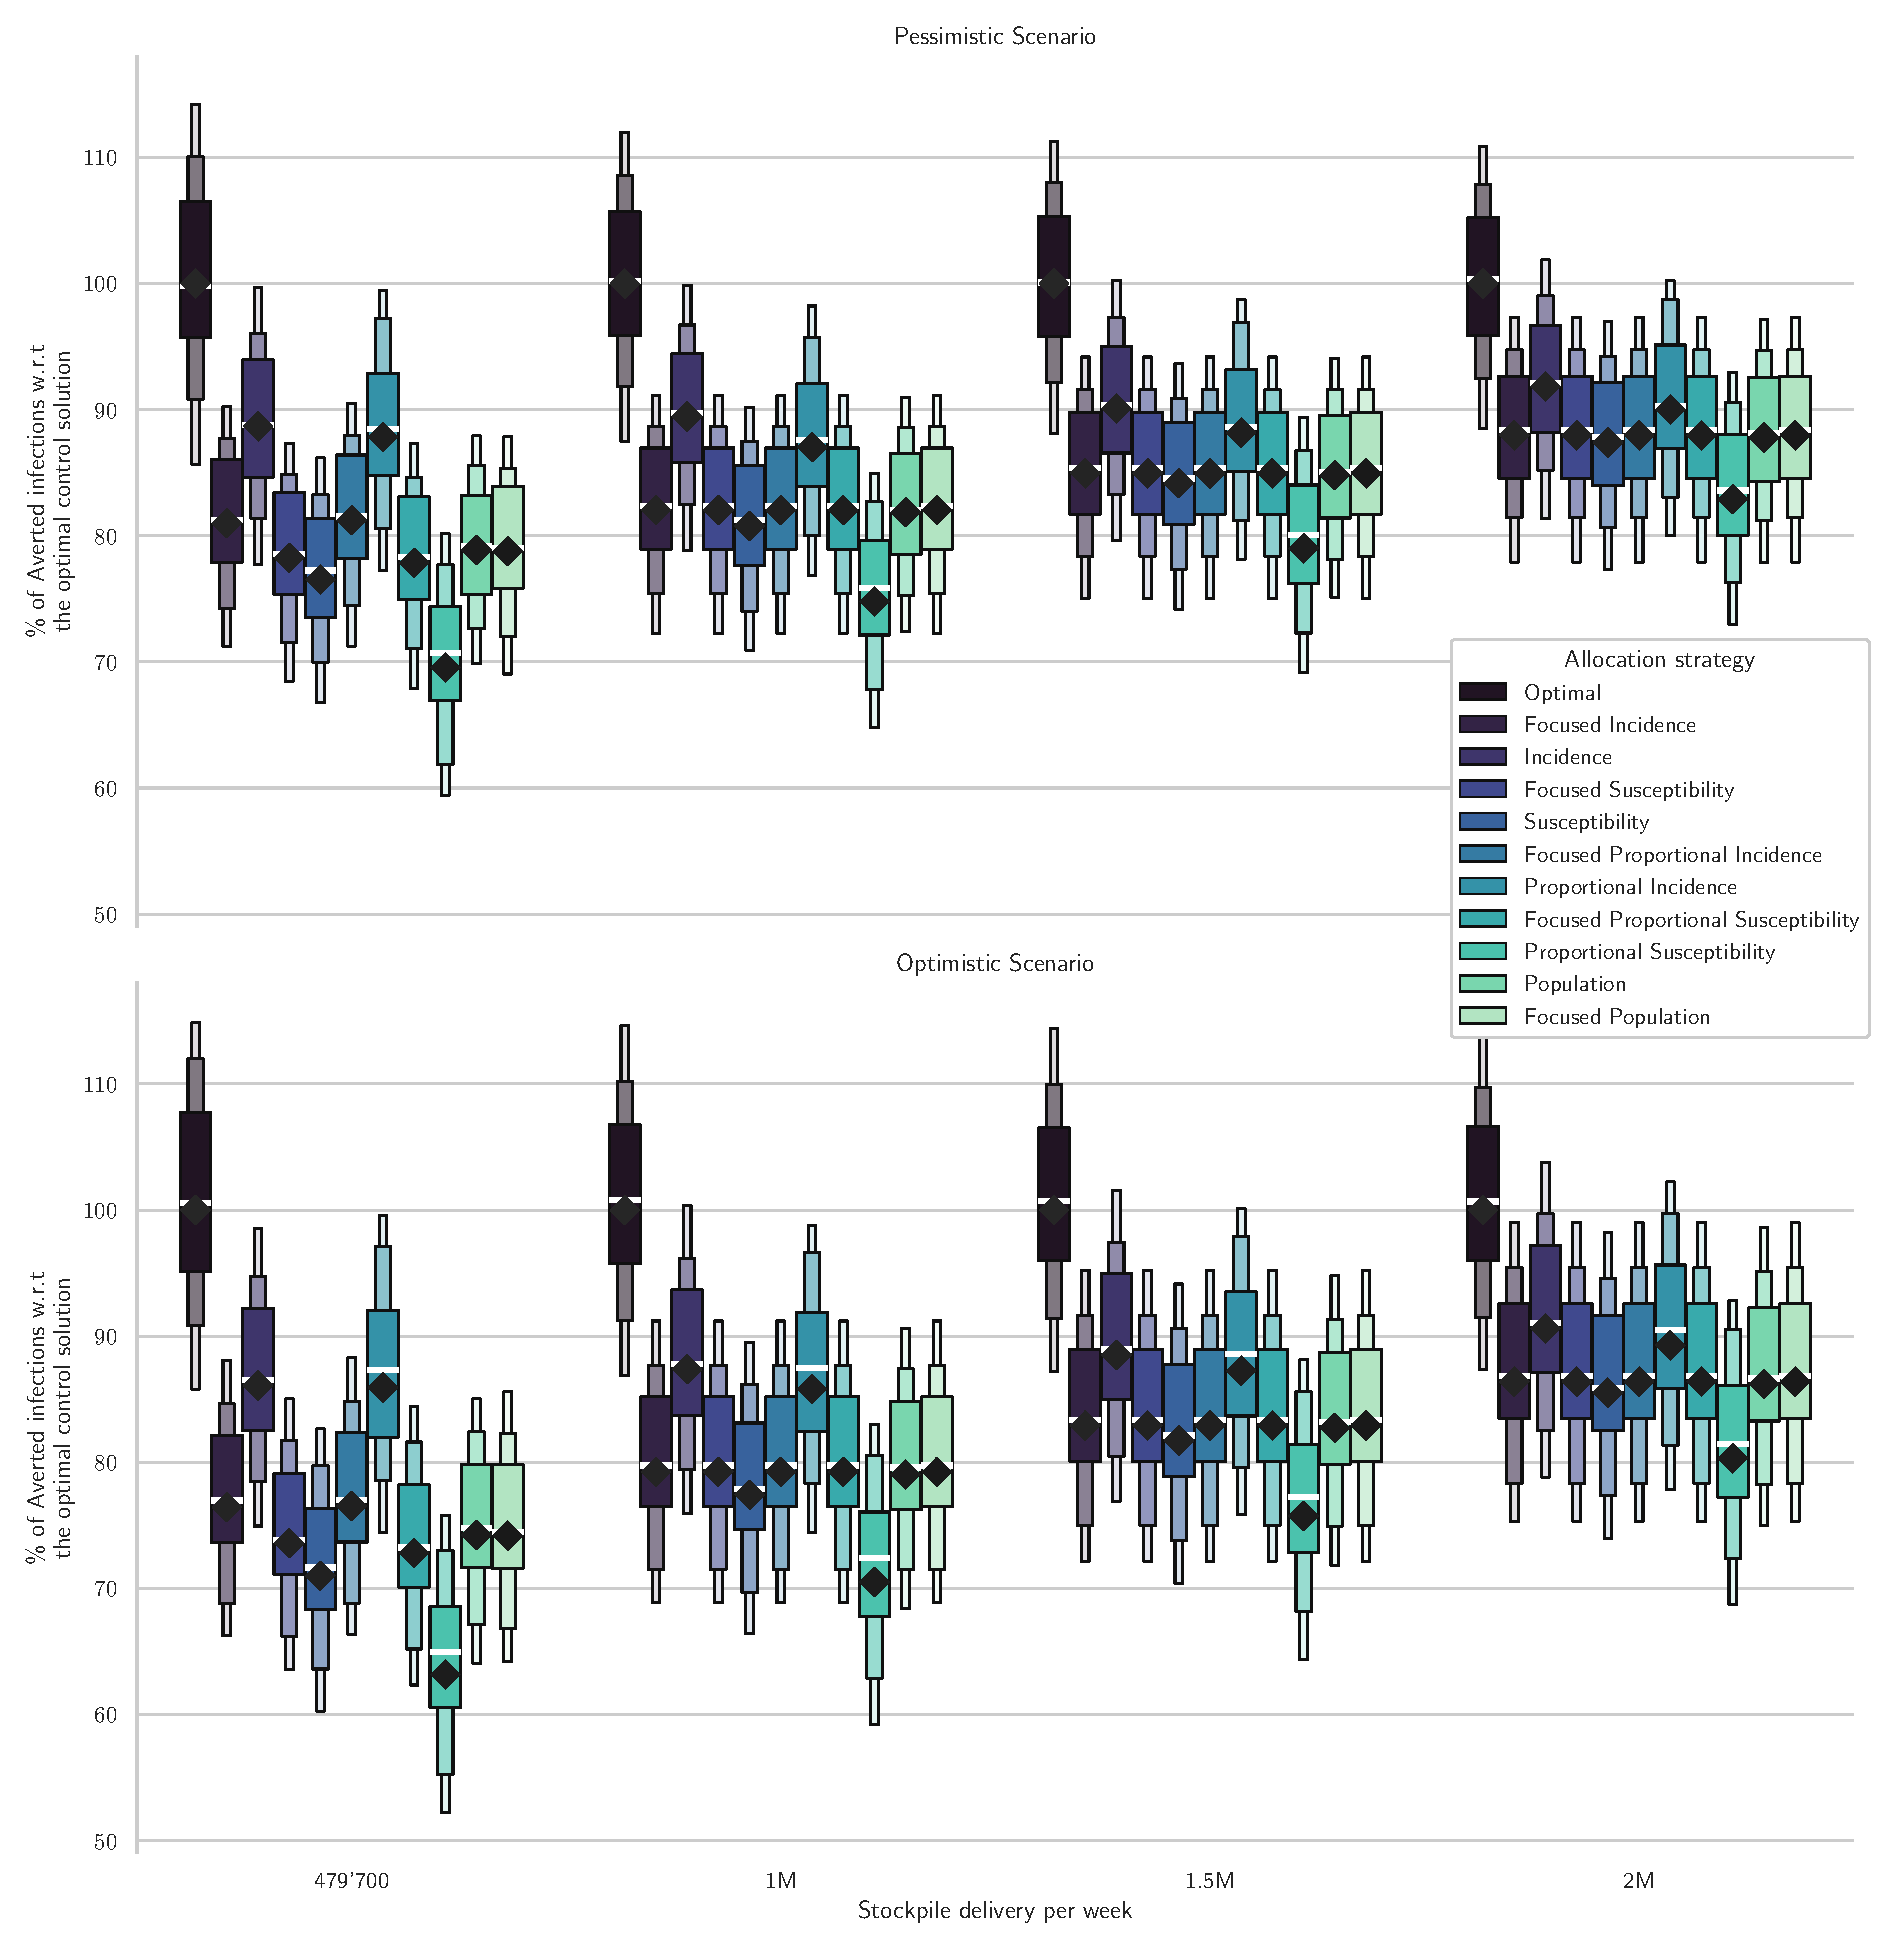
\includegraphics[width=0.9\textwidth]{fig_italy-ocp/figuresSI/scenarios_perturb_all_SI.pdf}
    \caption[Comparison of different allocation strategies]{Comparison of different allocation strategies. Percentages of averted infections per vaccine dose from January 11, 2021 to April 11, 2021 using different vaccine distribution strategies for the pessimistic (panel A) and the optimistic (panel B) scenario based on: the optimal solution, the spatial distribution of the population, the amount of susceptible individuals at the beginning of the vaccination campaign, and the projected disease incidence in the absence of control. A median realization of the modeled posterior is optimized (diamonds), and the performance is assesed on the whole posterior (box plots). The results are normalized by the number of averted infections in the optimized solution (see tab.~\ref{table:all_strat} for absolute values).}
    \label{fig:OC_comparison_all}
\end{fwfigure}


\begin{figure}[!ht]
    \centering
    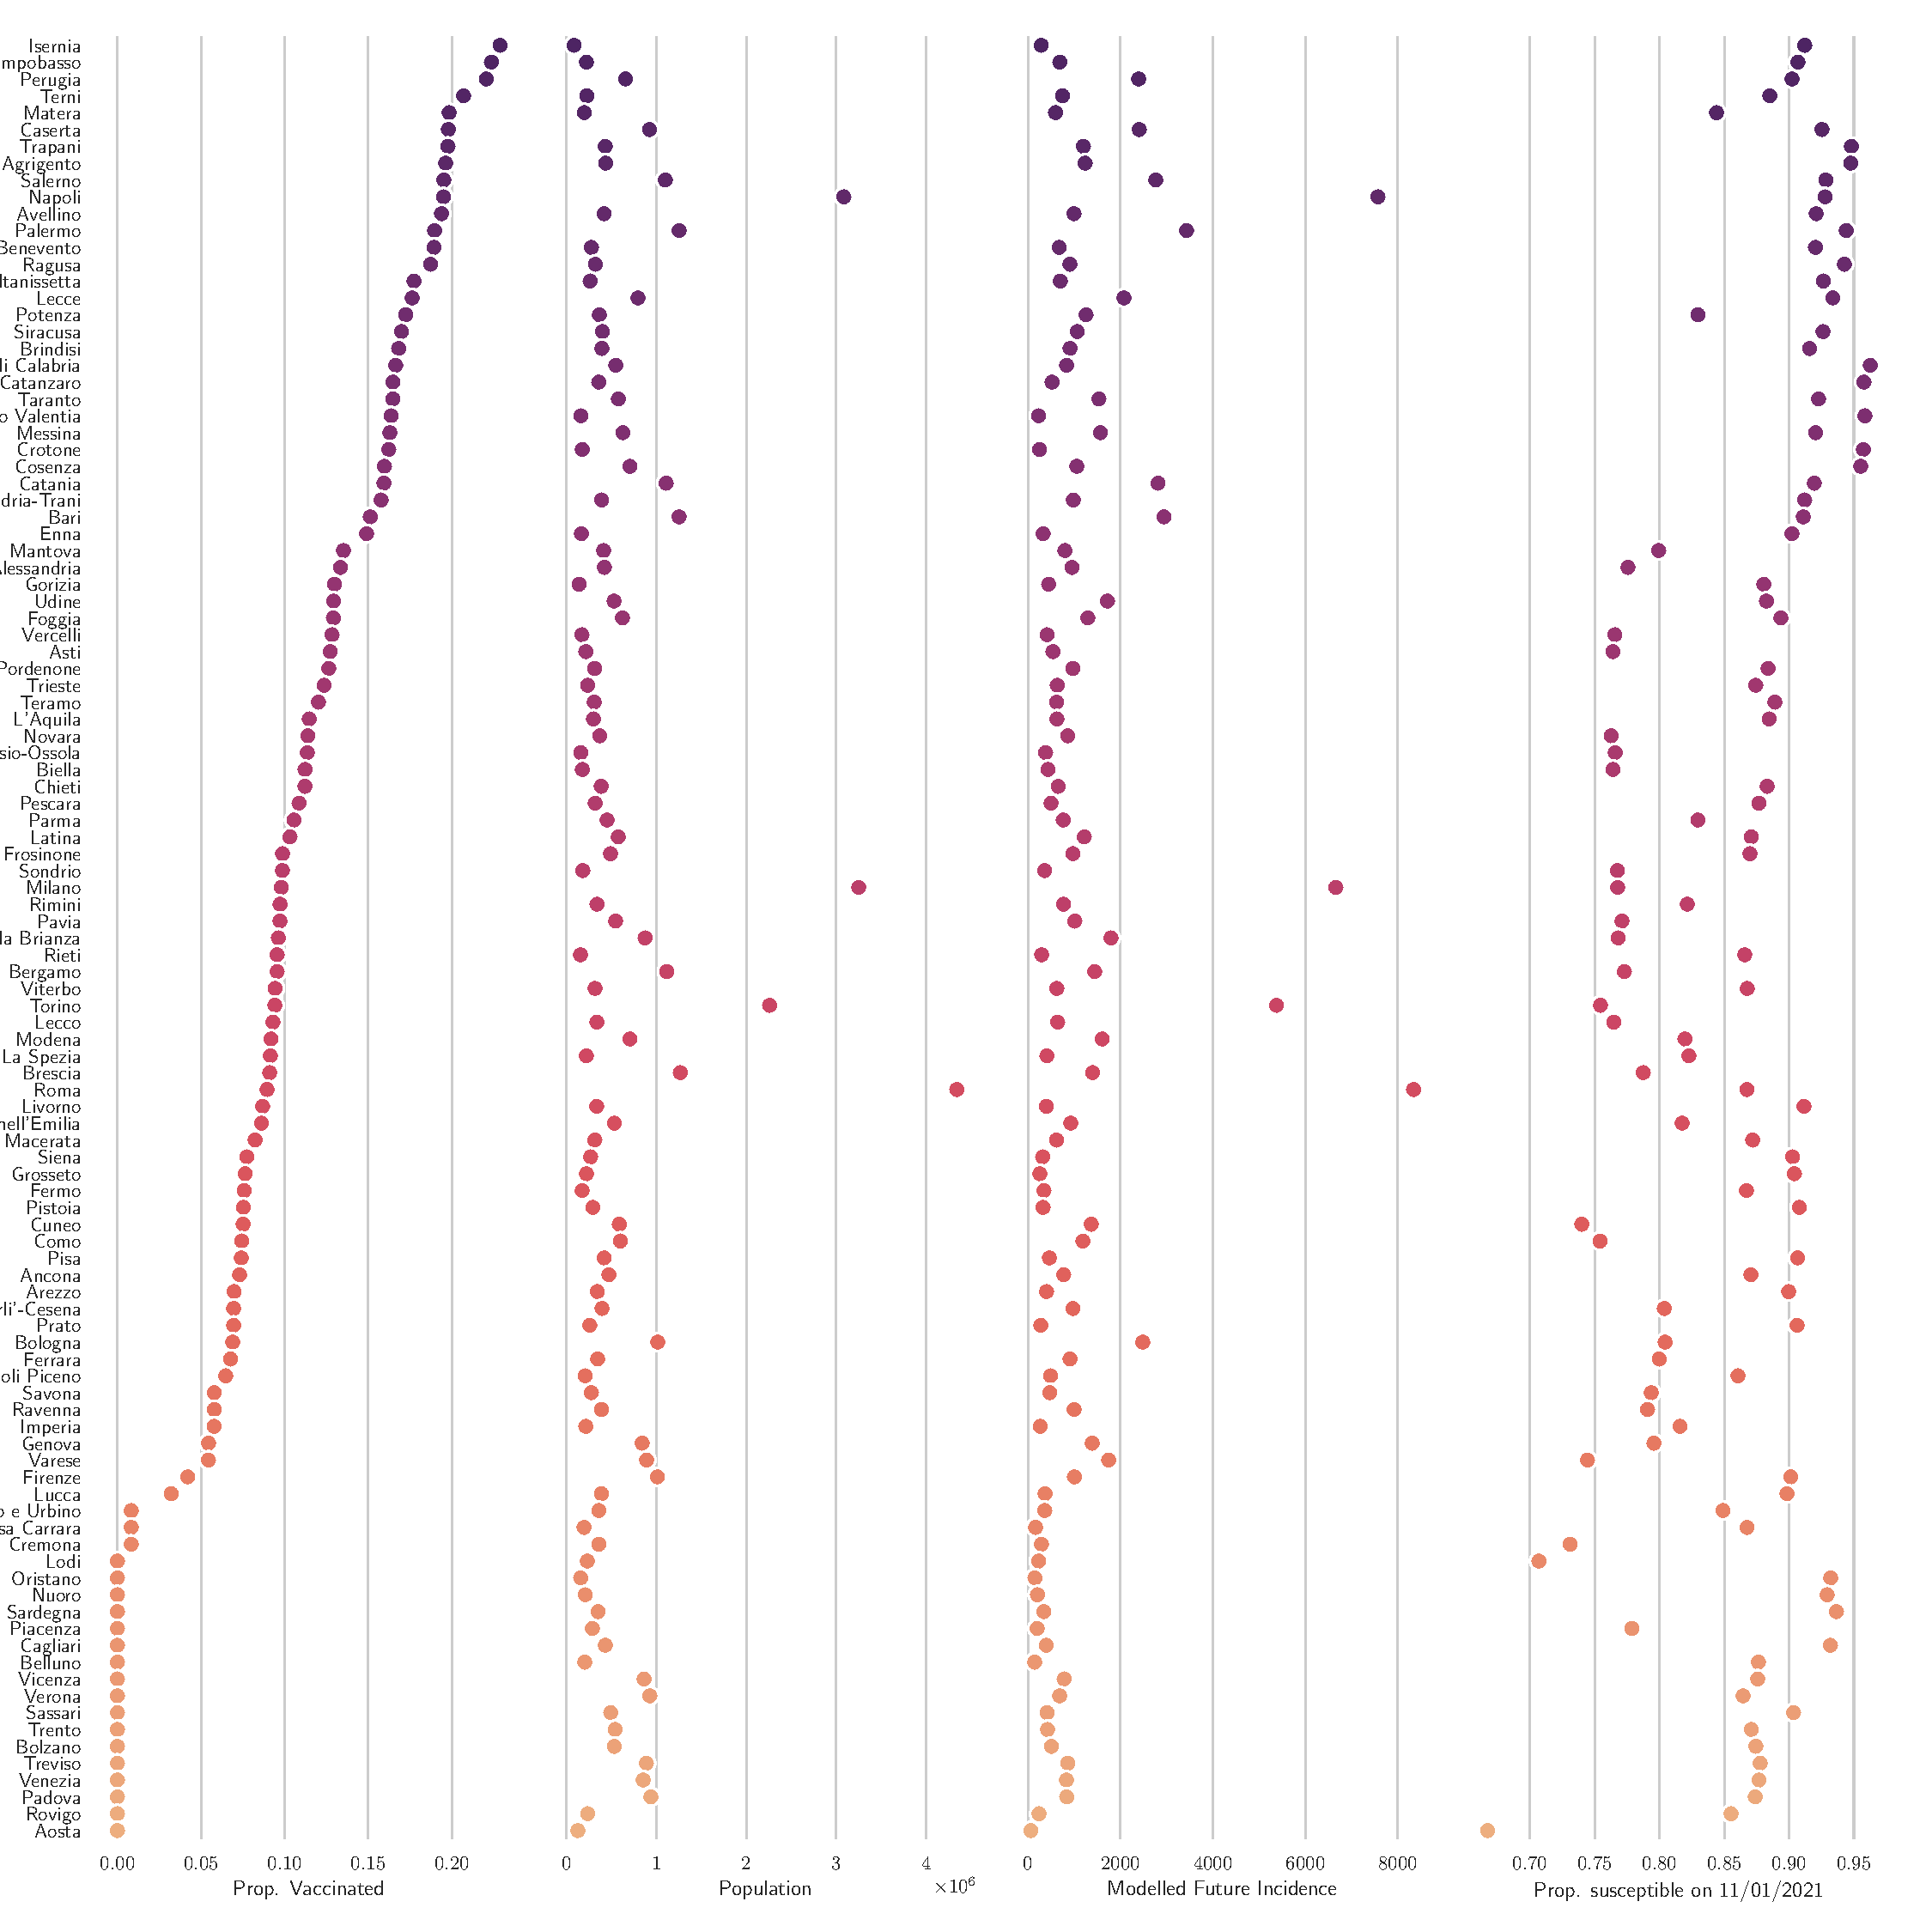
\includegraphics[width=\textwidth]{fig_italy-ocp/figuresSI/SI_scatter_Optimistic.pdf}
    \caption[Control and co-variates for the optimistic scenario]{Control and co-variates for the optimistic scenario with a stockpile delivery of 479'700 vaccine doses.}
    \label{fig:OC_scatter_optimistic}
\end{figure}

\begin{figure}[!ht]
    \centering
    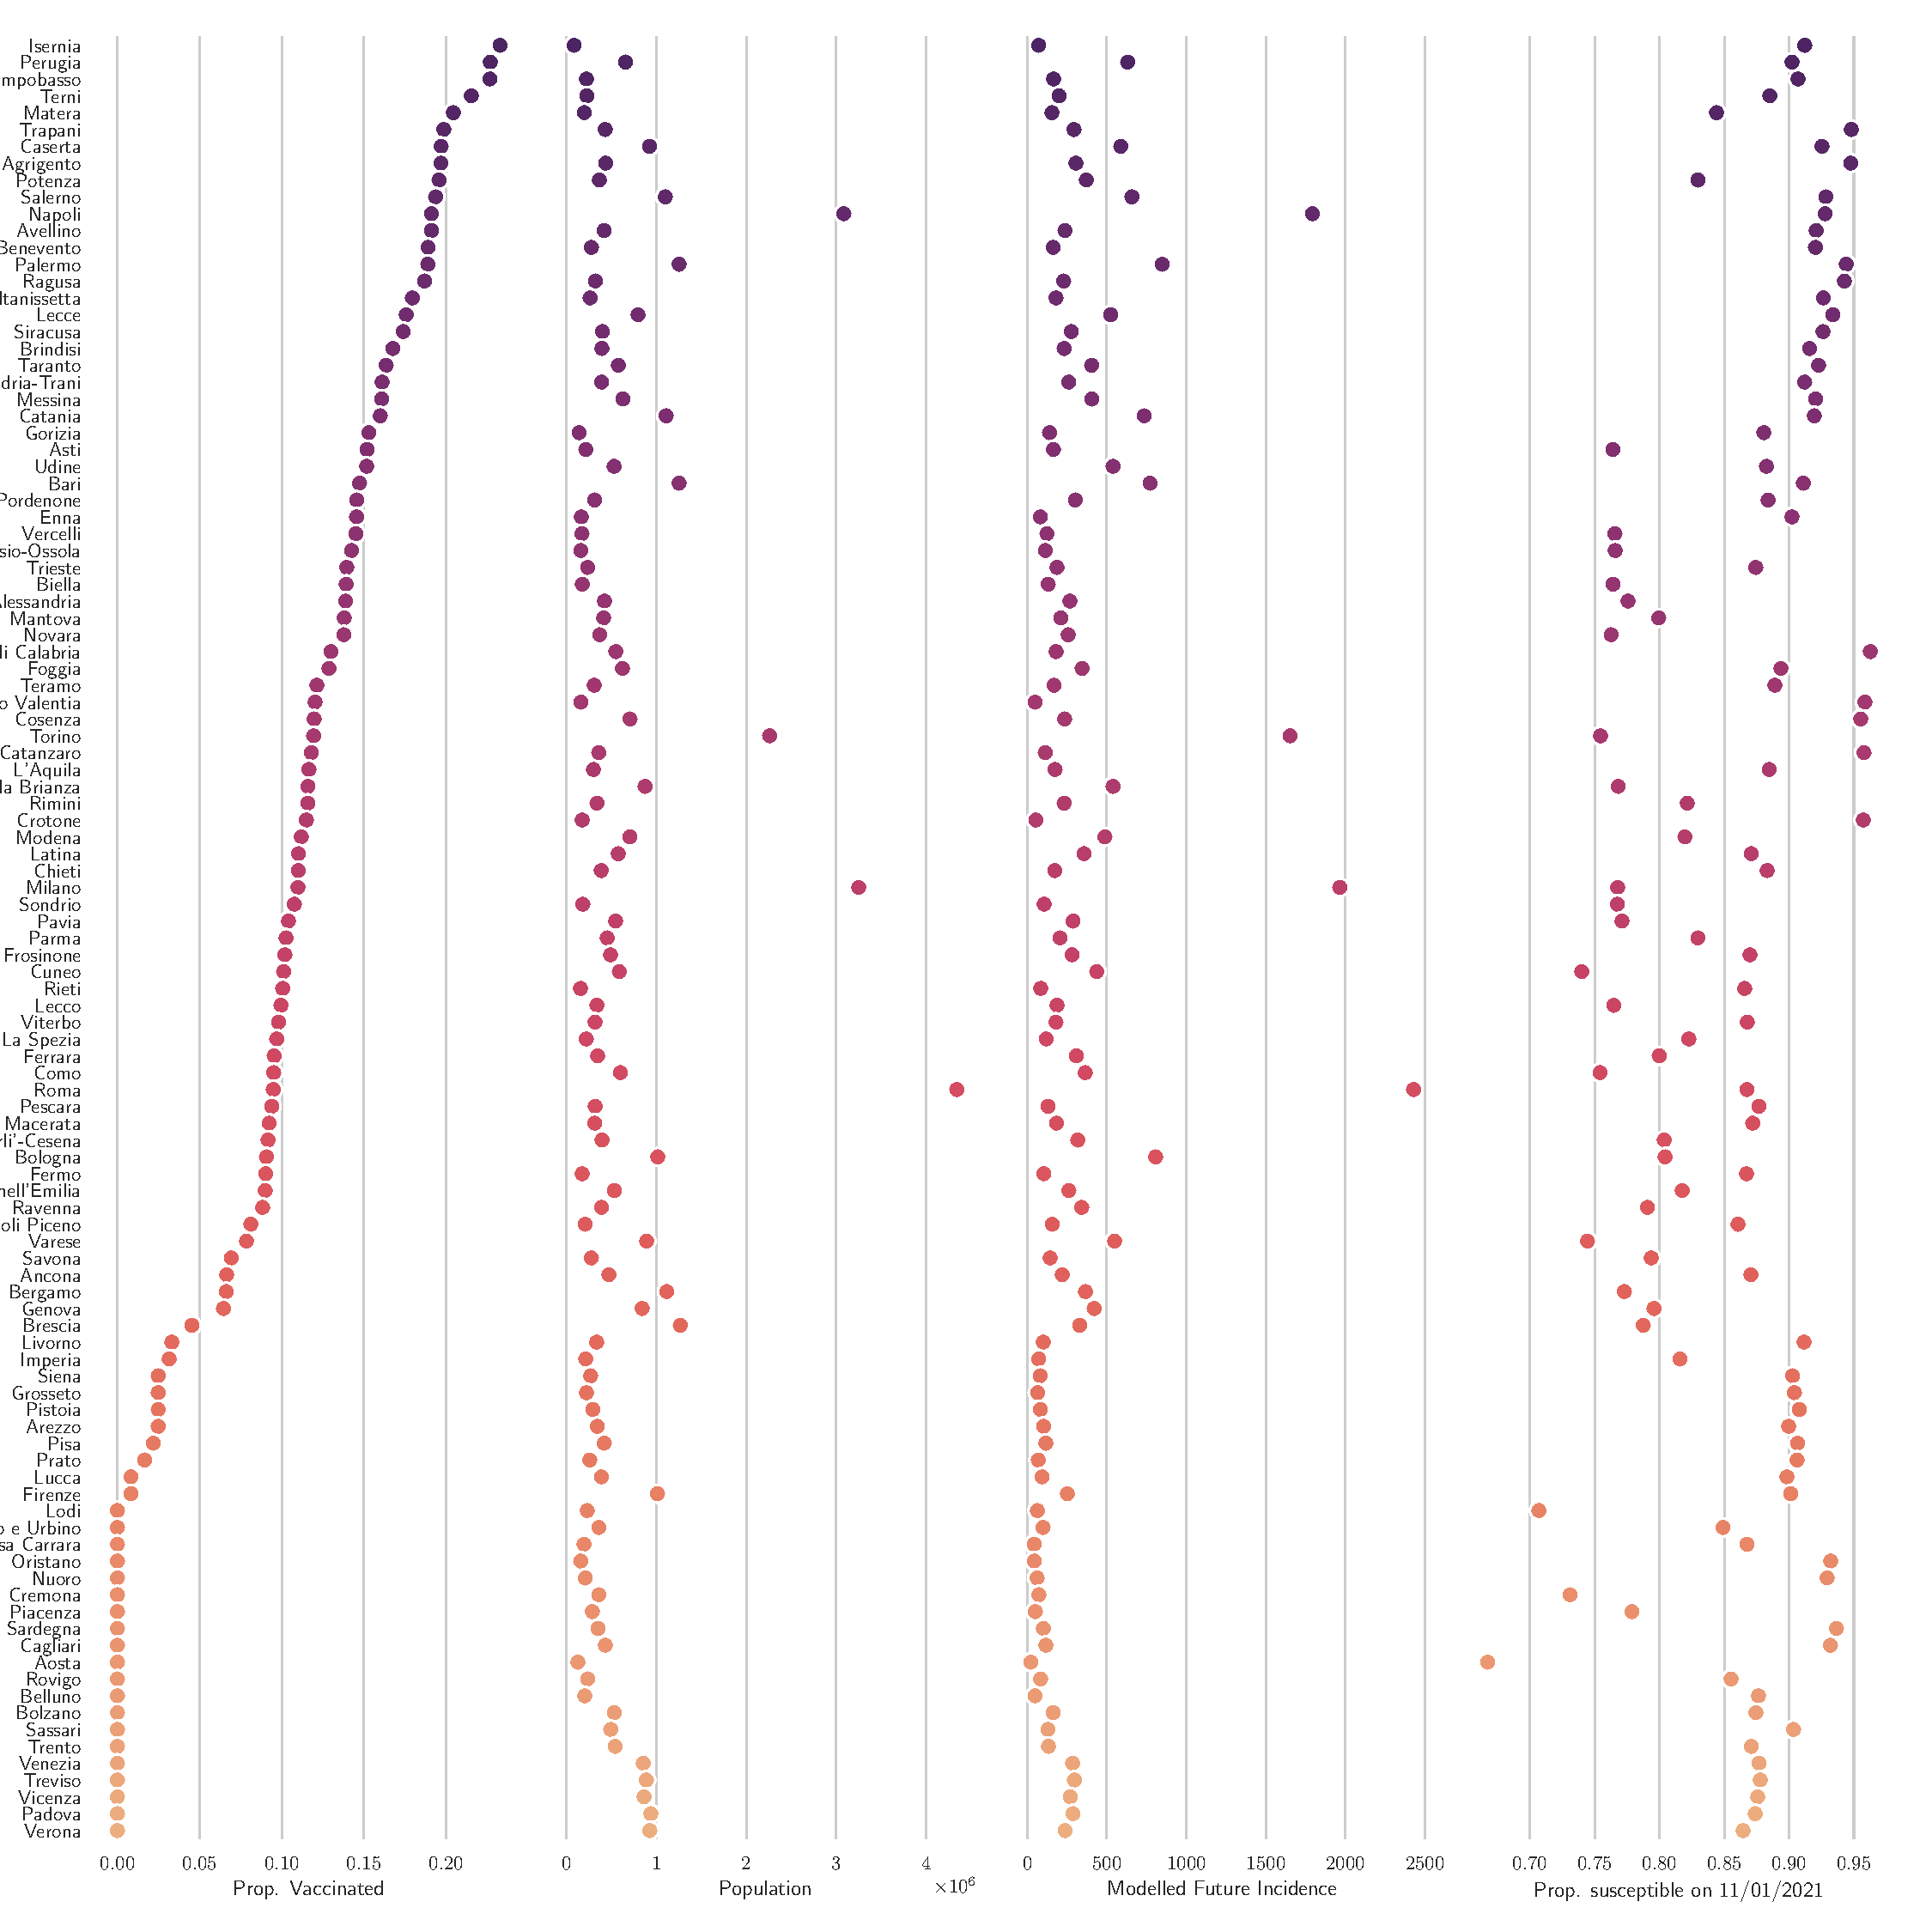
\includegraphics[width=\textwidth]{fig_italy-ocp/figuresSI/SI_scatter_Pessimistic.pdf}
    \caption[Control and co-variates for the pessimistic scenario]{Control and co-variates for the pessimistic scenario with a stockpile delivery of 479'700 vaccine doses.}
    \label{fig:OC_scatter_pessimistic}
\end{figure}

%\begin{figure}[!ht]
%    \centering
 %   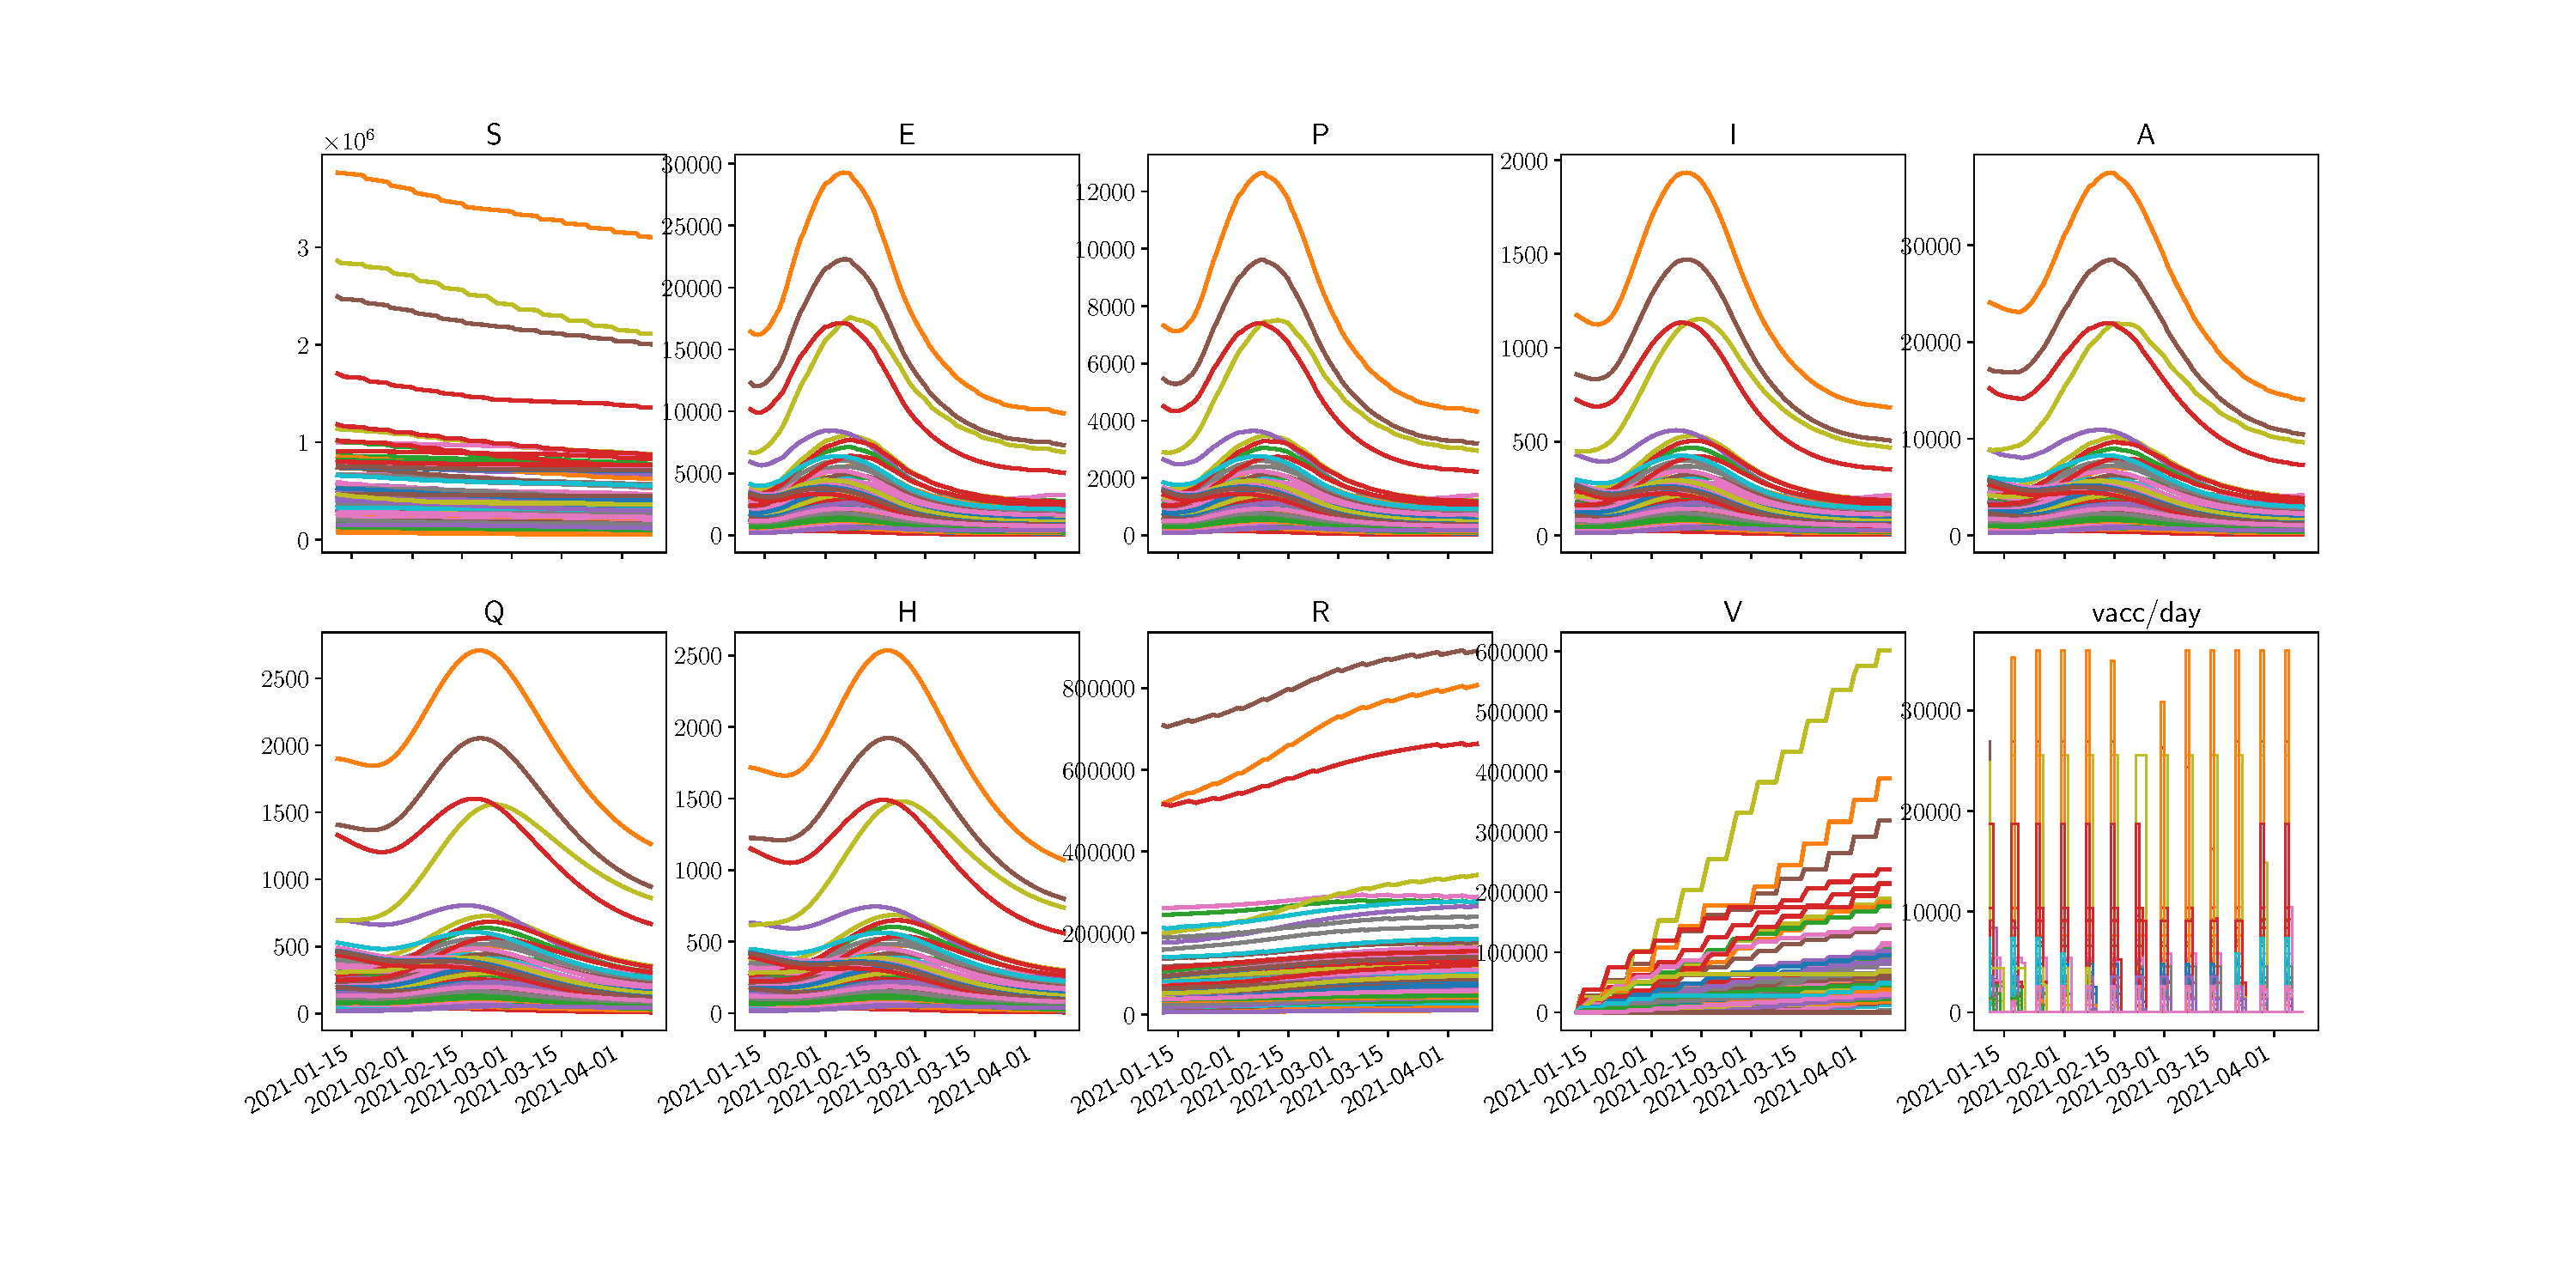
\includegraphics[width=\textwidth]{fig_italy-ocp/figuresSI/SI_all_states.pdf}
  %  \caption[Example of the dynamics in all compartments]{Example of the dynamics in all compartments for every node in the pessimistic scenario with a stockpile delivery of 479'700 doses. The lower right plot shows the control variable, the number of doses per day in each province.}
%    \label{fig:OC_ts_all}
%\end{figure}




